%************************************************
\chapter{Introductory Session}\label{ch:introduction}
%************************************************
\section{Objective}
To learn the art of observation and thereby analyse the morphological featurs of the wild type and mutant Drosophila melanogaster.

\section{Theory}
	\subsection{Morphology}
		Morphology is the study of form and structure of organisms.
		\par	
		Drosophila melanogaster is a small fly. It has two red coloured compound eyes, made up of 700-800 hexagonal units. It has two translucent wings, and a pair of halteres. It has a hairy body. It also has a pair of antennas. The abdomen is striped with visible differences between males and females.
	\subsection{Life Cycle}
		\begin{figure}[h]
			\begin{center}
				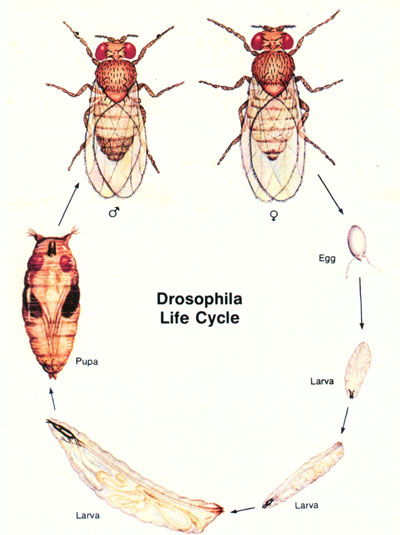
\includegraphics[width=.5\linewidth]{gfx/drosophila}
			\end{center}
		\caption[Drosophila Life Cycle]{Drosophila Life Cycle \citep{drosophila:lifecycle}}
		\end{figure}

		\par
		\begin{enumerate}
			\item Embryo: The first stage is from the fertilization of the egg, till the embryo hatches (under ideal conditions (at $25\,^{\circ}\mathrm{C}$), takes 12-16 hours), inside the mother. The insect starts as a single cell, and then develops into the larval form before it hatches.
			\item Larva: The second stage is from birth until the larva pupates. This stage is generally worm-like. It grows for about 4 days while \emph{molting} twice (into 2nd- and 3rd-instar larvae), at about 24 and 48 h after hatching. They feed on the micro-organisms that decompose the fruit, as well as on the sugar of the fruit itself, during this period.
			\item Pupa: this is the third stage, from pupation till eclosion. This stage is marked by reduced movement and often sealed with a cocoon. The metamorphosis takes about 4 days.
			\item Imago: In this stage, the holometabolous insects are adults and usually have wings and functioning reproductive organs.
		\end{enumerate}
		\marginpar{\Maggie Holometabolism: This term is used to describe the specific kind of insect development which includes all four life stages.} Holometabolic development gives the offspring a very unique advantage of not being forced to compete with the adults since they inhabit different ecological niches due to the morphological differences in the different stages of their life cycle.
	\subsection{Difference between Males and Females}
		\begin{figure}[h]
			\begin{center}
				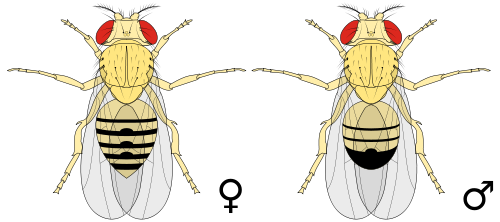
\includegraphics[width=.6\linewidth]{gfx/Male_Female_drosophila}
			\end{center}
		\caption[Male and Female Drosophila]{Male and Female Drosophila}
		\end{figure}

		\begin{enumerate}
			\item Females have a shorter life compared to males.
			\item On an average, females are larger than males (although not necessarily individually true)
			\item Males have a larger portion of their back black compared to females. However, this distinction is not very clear until they're mature.
			\item Males have sex-comb which is the most reliable distinguishing feature amongst males and females. It is present in the first leg.
		\end{enumerate}

\section{Experiment}
	We were divided into groups of three and each group was given a vial containing over 30 Drosophila melanogaster. Our objective was to analyse them under a stereo microscope and study their morphology within 45 minutes.
	\par
	My team consisted of Vivek Sagar (MS11017), Biplob Nandy (MS11004) and I (MS11003). The issue at hand was to focus a moving organism with the microscope. We came up with the following solution.
	\begin{aenumerate}
		\item Locate a cylindrical object with a small diameter.
		\item Use the object to push the cotton away from the walls of the container, while gradually moving into the container.
		\item Continue the process till a fly gets into the gap between cotton and the vial wall, upon occurrence of which, release the cotton to firmly hold the fly.
		\item This ensures that the fly has very restricted movements and is still alive.
	\end{aenumerate}
	\par
	This was followed by a discussion about the observations, after which we were told how to put the flies to ``sleep'', or more precisely, anaesthetising them. \marginpar{\Lisa After the flies recover their conciousness, their behaviour ceases to be normal.} The method was straight forward. It involved the use of ether, which inhibits neurological pathways in drosophila. The protocol followed was:
	\begin{aenumerate}
		\item Locate a funnel. At the terminal part of its conical region, attach a cotton ring.
		\item Add a few drops of the anaesthesia to the cotton.
		\item Now take an empty vial and place the funnel on its mouth, covering it completely.
		\item Locate the vial which contains the drosophila desired to be anaesthetised.
		\item Remove the cotton plug and instantly place the mouth of the vial on the funnel
		\item The drosophila will fall through the funnel into the empty vial, unconscious.
		\item Remove the funnel after a suitable duration.
	\end{aenumerate}
	One such unconscious fly's front leg was taken and focussed under a high power microscope and observed.
	\par
	And lastly, Mutants were setup for viewing under stereo microscopes and we were asked to observe them.
\section{Observations}
	\subsection{Coarse Focus}
		\begin{enumerate}
			\item Flies were of different size.
			\item There were 3 pairs of legs.
			\item All of them had Red coloured eyes.
			\item All had their abdomen striped with Yellow Brown and Black
			\item In most, there were 5 stripes.
		\end{enumerate}

	\subsection{Fine Focus}
		
		\subsubsection*{Observations of a particular fly}
			\begin{enumerate}
				\item 2 hair like protrusions from the head were observed. Most likely they were antennas.
				\item There were only 2 pairs of wings.
				\item Back colour was Yellowish Brown
				\item The body was shiny and globular.
			\end{enumerate}
		
		\subsubsection*{Observations of a different fly}
			\begin{enumerate}
				\item Hair like projections were visible on all three legs.
				\item Abdomen was white in colour.
				\item Halteres were observed.
			\end{enumerate}

		\subsubsection*{Observations of yet another fly}
			\begin{enumerate}
				\item Most of the body had black coloured hair, including the face.
				\item Legs had a hook like structure
				\item It seemed to be releasing a black shiny liquid
				\item Lines in the wings were distinctly visible (later told to be veins)
				\item Hexagonal eyes were visible. Could see the hexagonal elements.
				\item Could see a slightly darker circle in the eye (later told to be sensory nerves)
			\end{enumerate}

		\subsubsection*{Non-microscopic Observations}
			\begin{enumerate}
				\item The flies try to run \emph{away} from gravity.
				\item The flies run \emph{towards} light.
			\end{enumerate}
	\subsection{High Power Microscope}
		The sex comb was explicitly visible in the front leg.
	\subsection{Mutants}
		\begin{enumerate}
			\item Barred eyes
			\item Eye Colour
				\begin{aenumerate}
					\item White
					\item Orange
					\item Brown
				\end{aenumerate}
			\item Curly Wings
			\item Gray and Yellow Body
		\end{enumerate}
\section{Acknowledgements}
I thank both my team members, Biplob Nandy (MS11004) and Vivek Sagar (MS11017) for their contribution to the performance of the experiment. 